\subsection{Kontrolinterfacet}
I dette afsnit beskrives design og implementering af Kontrolinterfacet som lavet på baggrund af kravspecifikationen og systemarkitekturen. 

Designet af Kontrolinterfacet afspejler meget den generelle opbygning af systemet. Således er hvert element af systemet implementeret som en klasse. Derudover er der nogle hjælpeklasser. En oversigt over klasserne og deres ansvar kan ses i tabel \ref{tabel:ki-klasser}

Det gælder for VBTE-, SM- og Sensor-klasserne at når der efterspørges en af de værdier, klassen har ansvaret for, så benyttes RS232-objektet til at fremskaffe disse værdier ved hjælp af den serielle kommunikationsprotokol.


\begin{figure}[H]
\centering
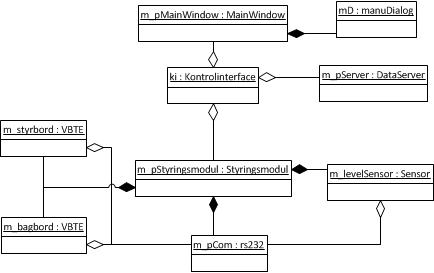
\includegraphics[scale=0.8]{billeder/Objektdiagram}
\caption{Oversigt over, og sammenhæng mellem, objekter i kontrolinterface-programmet}
\label{fig:objektdiagram}
\end{figure}


\begin{table}[H]
\centering
\begin{tabular}{| p{3cm}  p{11cm}|}
\multicolumn{2}{l}{{\Large Kontrolinterfacets klasser}} \\\hline
Kontrolinterface:&Programmets hovedklasse. Eksisterer for at rydde op i main-funktionen.\\\hline
DataServer:&Står for alt TCP-kommunikationen med databasen. Oprettes af KI-klassen\\\hline
Styringsmodul:&Oprettes af KI og opretter VBTE-, Sensor- og RS232klasserne.\\\hline
Sensor:&Oprettes af SM og er ansvarlig for hældningsværdien.\\\hline
VBTE:&Der eksisterer et VBTE-objekt for hvert fysisk VBTE-modul. Det er objektets ansvar at holde styr på værdierne for sit VBTE-modul.\\\hline
RS232:&Objektet oprettes af SM-klassen og VBTE- og Sensorobjekterne har en delt association til den. Objektet har ansvaret for kommunikationen med det fysiske SM-modul. Objektet formidler sig på en protokol forstået den kommunikationsansvarlige kode på SM-modulet. Protokollen kan ses i dokumentet for det detaljerede softwaredesign.\\\hline

MainWindow:&Oprettes af KI-klassen. Kontrollerer og overvåger den grafiske brugergrænsefalde.\\\hline
manudialog:&Oprettes af MainWindow og styrer den dialog, der fremkommer når man ønsker en manuel hældningsregulering.\\\hline
\end{tabular}
\caption{Kontrolinterfacets klasser}
\label{tabel:ki-klasser}
\end{table}

\subsubsection{Grafisk brugergrænseflade}
I denne sektion vil der kort blive gennemgået det vigtigste vindue i den grafiske brugergrænseflade; hovedvinduet. En gennemgang af de resterende vinduer vil kunne findes i Softwaredesign Appendix A: Kontrolinterface.
På figur \ref{fig:hovedvindue} er hovedvinduet vist. Her er vinduets elementer indrammet. En beskrivelse af hvert element vil kunne findes i tabel \ref{tabel:ki-elementer}.

\begin{figure}[H]
\centering
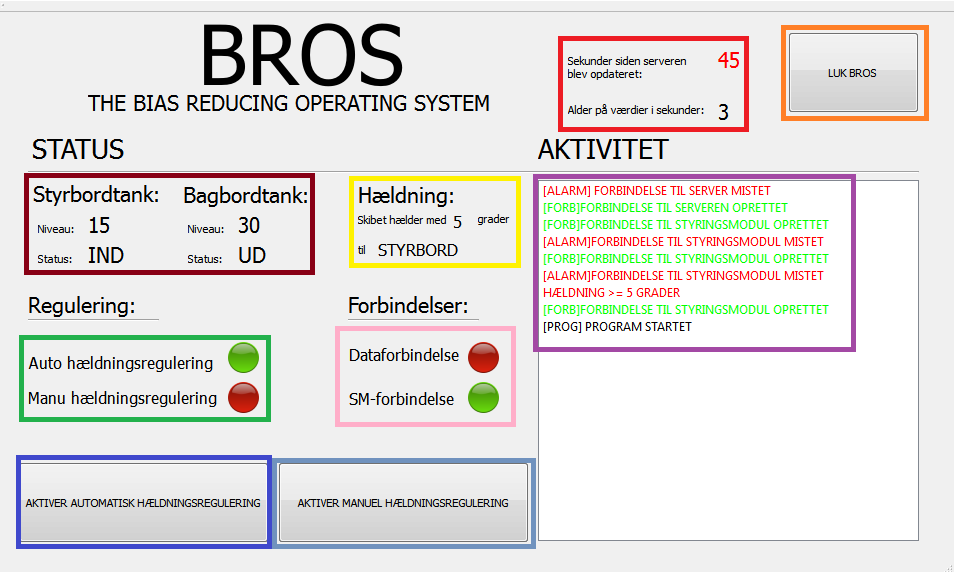
\includegraphics[width=0.5\textwidth]{billeder/hovedvindue}
\label{fig:hovedvindue}
\caption{På figuren ses hovedvinduet for Kontrolinterface-programmet}
\end{figure}


\begin{table}[htbp]
\label{tabel:ki-elementer}
\begin{tabular}{l p{10cm}}
\multicolumn{2}{l}{{\Large Hovedvinduets elementer}} \\\hline
\hline
\textcolor{red}{\textbf{1: Forsinkelse i sekunder}}
&Det øverste tal fortæller tiden i sekunder siden serveren sidst er blevet opdateret succesfuldt.
Nedenunder udskrives tiden i sekunder siden værdierne i boks tre og fire er blevet opdateret.\\

\textcolor{Orange}{\textbf{2: Nedlukningsknap}}
&Anvendes til at lukke programmet. Programmet åbner dialogen som ses i \ref{fig:lukkevindue}\\

\textcolor{brown}{\textbf{3: Vandballasttankene}}
&Her kan status for vandballasttankene aflæses. Niveauet er hvor fyldt tanken er angivet i procent. Hvis niveauet er over 70\% skrives tallet med rødt.
Status angiver vandets flow i tanken: IND/UD/LUKKET.\\

\textcolor{yellow}{\textbf{4: Hældningssensor}}
&Værdien for hældningen af skibet angives i antal grader og i hvilken side skibet hælder.\\

\textcolor{green}{\textbf{5: Reguleringsstatus}}
&Her angives hvorvidt automatisk eller manuel hældningsregulering er aktiveret. Der vil altid kun være en og kun en af disse aktiveret. Derfor vil der altid være en rød og en grøn indikator tændt. I dette eksempel er den automatisk hældningsregulering aktiveret.\\
\textcolor{pink}{\textbf{6: Forbindelser}}
&Indikerer hvorvidt der er forbindelse til Styringsmodulet og serveren. Dataforbindelse er rød hvis det ikke lykkedes at oprette forbindelse til serveren ved sidste forsøg.
SM-forbindelse er rød hvis det ikke lykkedes at få de ventede svar fra Styringsmodulet.
I denne situation er der forbindelse til styringsmodulet, men ikke serveren.\\

\textcolor{blue}{\textbf{7: Automatisk reguleringsknap}}
&Ved tryk på denne knap vil man komme til dialogen på \ref{fig:aktiver_auto} såfremt automatisk styring ikke er aktiveret. Hvis den er aktiveret og man trykker på knappen vil dialogen på figur \ref{fig:auto_aktiveret} fremkomme.\\

\textcolor{BlueGreen}{\textbf{8: Manuel reguleringsknap}}
&Bringer dig til dialogen på figur \ref{fig:manuelregulering}\\

\textcolor{purple}{\textbf{9: Aktivitetslog}}
&Her udskrives vigtige hændelser i programmet med farvekoder. I dette eksempel kan det ses hvordan alarmer skrives med rødt og oprettede forbindelser skrives med grønt.\\

\end{tabular}
\end{table}